\documentclass[twoside]{article}
\usepackage{amssymb}
\usepackage{amsmath}
\usepackage{amsthm}
\usepackage{algorithm}
\usepackage{algpseudocode}
\usepackage{caption}
\usepackage{subcaption}
\usepackage{enumerate}% http://ctan.org/pkg/enumerate
\usepackage{pgfplots}
\usepackage{multicol}
\usepackage[hmarginratio=1:1,top=32mm,columnsep=20pt]{geometry}
\usepackage{fullpage}
\usepackage{pdflscape}
\usepackage{setspace}
\usepackage{url}
\usepackage{tikz}
\usetikzlibrary{tikzmark}
\usepackage{color}
\usepackage{pgfplots}
\usepackage{bm}
\usepackage{tikz-cd}
\pgfplotsset{compat=newest}
\usepgfplotslibrary{fillbetween}
\usepackage[toc,page]{appendix}
%\usepackage[shortlabels]{enumitem}\usepackage{draftwatermark}

\usetikzlibrary{arrows.meta,
                calc, chains,
                patterns,
                patterns.meta,
                fit,
                quotes,
                positioning,
                shapes.geometric,
                shapes.misc,
                automata
                }
%Flowchart Tikzset
\tikzset{
   recbox/.style = {
         rectangle,
         draw, 
         align = center, 
         text badly centered,
         inner sep = 6 pt,
         font=\footnotesize,
         line width = 0.3mm,
      },
      circlebox/.style = {
         rounded rectangle,
         draw, 
         align = center, 
         text badly centered,
         inner sep = 7 pt,
         font=\large,
         line width = 0.5mm,
      },
      roundbox/.style = {
         rectangle,
         draw, 
         align = center, 
         rounded corners,
         text badly centered,
         inner sep = 6 pt,
         font=\large,
         line width = 0.5mm,
      },
     box1/.style = {
         rectangle,
         draw, 
         align = center, 
         text badly centered,
         inner sep = 6 pt,
         font=\large,
         line width = 0.5mm,
         minimum width = 30mm,
         minimum height = 7mm,
      },
    papLine/.style = {
         draw,
         -stealth,
         font=\ttfamily,
         line width = 0.5mm,
      },
      }
%end flowcahrt tikz set   

%Colors 
\definecolor{darkgreen}{rgb}{0.01, 0.75, 0.24}
\definecolor{shaded_green}{RGB}{151, 194, 157}

\newcommand{\quotes}[1]{``#1''}

\theoremstyle{plain}% default
\newtheorem{theorem}{Theorem}[section]
\newtheorem{lemma}[theorem]{Lemma}
\newtheorem{proposition}[theorem]{Proposition}
\newtheorem*{corollary}{Corollary}

\theoremstyle{definition}
\newtheorem{definition}{Definition}[section]
\newtheorem{example}{Example}[section]
\newtheorem{exercise}[example]{Exercise}

\theoremstyle{remark}
\newtheorem*{rem}{Remark}
\newtheorem*{note}{Note}
\newtheorem{case}{Case}

\begin{document}
\parindent=0in
\parskip=12pt

%\SetWatermarkText{Draft}
%\SetWatermarkScale{5}

\title{
  Addendum to Relative Probability on Finite Sample Spaces \\
  \large{
    Using an Open Patch System to Define a Topology
  }
}

\author{Max Sklar\\ Local Maximum Labs \\ DATE HERE}
\date{}

\maketitle
\thispagestyle{empty}

\begin{abstract}
This is a quick addedum to Relative Probability of Finite Sample Spaces, where an alternative definition of the topology is presented.
\end{abstract}

\section{Relative Probability Space}
\label{section:new_relative_prob}

In Relative Probability on Finite Sample Spaces\cite{paper}, we looked at the set of relative probability functions - or more specifically totally comparable RPFs - as a space and proved its compactness. That proof was done by embedding it into a Euclidean space, whereas in this addendum we will go through a different construction for the topology of totally comparable RPFs. This construction is unneccesary, but perhaps it will be of interest to some readers. The author feels that it is a more natural definition, and may be of use in deriving better proofs, and also better schemes for representing regions of RPF space.

We being by reiterating some of the definitions from before\cite{paper}.

Let \(\Omega\) be a finite set of outcomes in a probabilistic system, and let \(P\) be a function that assigns a magnitude \(\mathbb{M} = [0, \infty]\) to every pair of outcomes.
\[P: \Omega \times \Omega \rightarrow \mathbb{M}\]

\begin{definition}
\label{def:fundamental_laws}
\(P\) is a \textit{totally comparable relative probability function} (RPF) on \(\Omega\) if \(P\) obeys the following 3 fundamental axioms:

\begin{enumerate}[(i)]
\item The \textit{identity axiom}: \(P(h, h) = 1\)
\item The \textit{inverse axiom}: \(P(h_1, h_2) = P(h_2, h_1)^{-1}\)
\item The \textit{composition axiom}: \(P(h_1, h_3) :\cong P(h_1, h_2) \cdot P(h_2, h_3)\)
\end{enumerate}

\end{definition}

\(P\) is considered \textit{totally mutually possible} when \(P: \Omega \times \Omega \rightarrow (0, \infty)\).

\begin{definition}
Let \(\text{RPF}(K)\) be the set of all totally comparable RPFs on \(\Omega = \{0, 1, ..., K-1\}\)
\end{definition}

\section{Composing Relative Probability Functions}

Let \(P_0, P_1, ..., P_{K-1}\) be relative probability functions on outcome spaces \(\Omega_0, \Omega_1, ..., \Omega_{K-1}\) respectively.

We can combine all of these relative probability functions together with a top level probability function \(P_\top\) (pronounced \quotes{P-Top}) with outcome space \(\Omega_\top = \{\Omega_0, \Omega_1, ... \Omega_{K- 1}\}\) as a weighted mixture of all \(P_k\).

We create a new relative probability function \(P\) acting on outcome space \(\Omega = \Omega_0 \cup \Omega_1 \cup \dots \Omega_{K-1}\) with the following rules:

\begin{itemize}
\item If the two outcomes fall under the same component, then their relative probabilities do not change:

\begin{equation}
\label{rpf_composition_same_branch}
P(h_{k, i}, h_{k, j}) = P_k(h_{k, i}, h_{k, j})
\end{equation}

\item If the two outcomes fall under different components, then their relative probabilities are given as follows.

\begin{equation}
\label{eq:rpf_composition_different_branch}
P(h_{k_1, i}, h_{k_2, j}) = P_{k_1}(h_{k_1, i}, \Omega_{k_1}) \cdot  P_{\top}(\Omega_{k_1}, \Omega_{k_2}) \cdot P_{k_2}(\Omega_{k_2}, h_{k_2, j})
\end{equation}
\end{itemize}

\section{Topology and Limits in Relative Probability Space}
\label{section:topology}

In \cite{paper}, we established a topology on \(\text{RPF}(K)\) by embedding it into Euclidean space, and demonstrated its compactness. Here we give an alternative topology that defines the open sets directly. This starts with finding a \textit{basis of open sets}.

The notion of an open set changes when a topological space is restricted to a lower dimention. For example, on the real number line \(\mathbb{R}\), the open interval (0, 1) is an open set. However, once it is embedded into \(\mathbb{R}^2\), it is now a line segment in a plane and no longer open (see figure \ref{fig:sub_topology}). It can be thought of as the restriction of an open set on \(\mathbb{R}^2\) to \(\mathbb{R}\). For example, the set \(\{(x, y): x \in (0, 1)\;  \text{and}\;  y \in (-\epsilon, +\epsilon)\}\) given an \(\epsilon > 0\) is such an open set on \(\mathbb{R}^2\).

\begin{figure}[h]
\centering
\resizebox{0.4\textwidth}{!}{
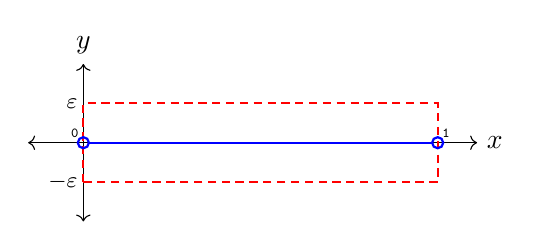
\begin{tikzpicture} %episilon diagram
\draw[<->] (-0.7,0)--(5,0) node[right] {\(x\)};
\draw[<->] (0,-1,0)--(0,1) node[above] {\(y\)};
\draw[densely dashed,red,thick] (0,-0.5) rectangle (4.5,0.5);
\draw[draw=blue,thick] (0,0) circle (2pt) node[above left=-0.1,font=\ttfamily\tiny] {0};
\draw[draw=blue,thick] (4.5,0) circle (2pt) node [above right=-0.1,font=\ttfamily\tiny] {1};

\node[left=-0.05,font=\ttfamily\footnotesize] at (0,-0.5) {\(-\varepsilon\)};
\node[left=-0.05,font=\ttfamily\footnotesize] at (0,0.5) {\(\varepsilon\)};
\node[circle,inner sep=1pt] at (0,0) (0){};
\node[circle,inner sep=1pt] at (4.5,0) (1){};
\path[draw,blue,thick] (0)--(1);
\end{tikzpicture}
}
\caption{The small box that is the interior of the dotted rectangle is an open set in \(\mathbb{R}^2\), and therefore its restriction to \(\mathbb{R}\) - the line segment - is an open set in \(\mathbb{R}\). But the line segment is not open in \(\mathbb{R}^2\).}
\label{fig:sub_topology}
\end{figure}

Likewise, an open set on \(\text{RPF}(K)\) will not be an open set on \(\text{RPF}(K+1)\).

Starting with \(\text{RPF}(2)\), we find a totally comparable RPF that corresponds 1:1 with the magnitude space.

\begin{theorem}
Let \(\Omega = \{0, 1\}\) have two elements, with relative probability function \(P\). Then, \(P\) is completely determined by \(P(0, 1)\).
\end{theorem}

\begin{proof}
Let \(q = P(0, 1)\). By the inverse symmetric property, \(P(1, 0) = q^{-1}\). These values completely determine \(P\) on the outcome level.
\end{proof}

This gives us both a topology and a compactness proof for \(\text{RPF}(2)\) because it is isomorphic to \(\mathbb{M}\). Its basis for open sets are the open intervals of \(\mathbb{M}\), including those intervals that include 0 and \(\infty\). For \(K > 2\), we will need more powerful tools.

\subsection{Open Patches}

The set of open patches will be a basis for the open sets on \(\text{RPF}(K)\). Open patches come in several flavors.

\begin{definition}
An \textit{interior open patch} of \(\text{RPF}(K)\) is one of the following:

\begin{enumerate}
  \item If \(K = 2\), a subset parameterized by an interior open interval of magnitudes. \(\{P | a < P(h_1, h_2) < b\}\) for some \(a, b \in \mathbb{M}\) 
  \item If \(K > 2\), a composition of interor patches with composing function \(P_{\top}\) also being an interior patch.
\end{enumerate}
\end{definition}

Interior open patches contain only totally mutually possible functions as illustrated in figure \ref{fig:interior_open_patch}.

\begin{figure}[h]
\centering
\resizebox{0.4\textwidth}{!}{
\begin{tikzpicture}
\node {\(P_\top\)} [sibling distance = 3cm]
  child {node {\(P_0\)}  [sibling distance = 3cm]
    child {node {A}}
    child {node {B}}
  }
  child {node  {C}};
\end{tikzpicture}
}
 \hspace{3em}
\resizebox{0.4\textwidth}{!}{
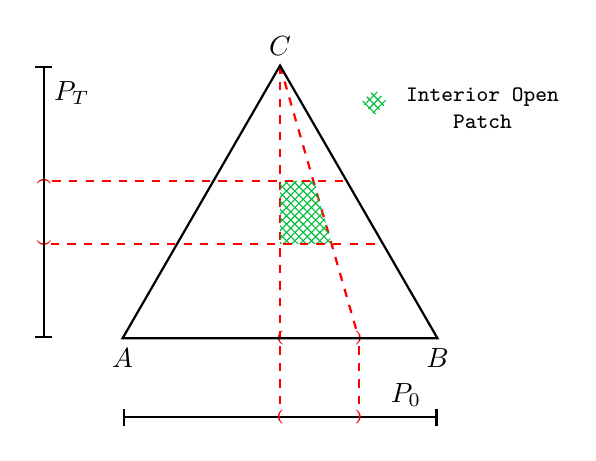
\begin{tikzpicture} %Triangle 3
\draw[thick, dashed,red] (0,{2*sqrt(3)})--(1,0) node [font=\tiny\bf] {)};
\draw[thick, dashed,red] (0,{2*sqrt(3)})--(0,0) node [font=\tiny\bf] {(};
\path[draw=none,pattern=crosshatch, pattern color=darkgreen] (0,1.2)--(0.66,1.2)--(0.43,2)--(0,2)--cycle;

\node[rectangle,rotate=45,draw=none,pattern=crosshatch, pattern color=darkgreen] at (1.2,3) (P){};

\node(Q)[rectangle,draw=none,align=center,below right=-0.3 and 0.1 of P,font=\ttfamily\footnotesize] {Interior Open\\ Patch};

\draw[thick] (-2,0)--(2,0)--(0,{2*sqrt(3)})--cycle;

\node (A) at (-2,0) [below] {\(A\)}; 
\node (B) at (2,0) [below] {\(B\)}; 
\node (C) at (0,{2*sqrt(3)}) [above] {\(C\)}; 

\draw[thick, dashed,red] (0.8,2)--(-3,2) node[font=\tiny\bf,rotate=90] {)};
\draw[thick, dashed,red] (1.2,1.2)--(-3,1.2) node[font=\tiny\bf,rotate=90] {(};

\draw[thick, dashed,red] (1,-0.1)--(1,-0.9);
\draw[thick, dashed,red] (0,-0.1)--(0,-0.9);

\draw[thick,|-|] (-3,0)--(-3,{2*sqrt(3)}) node[right,pos=0.9] {\(P_{T}\)};

\draw[thick,|-|] (-2,-1)--(2,-1) node[above,pos=0.9] {\(P_{0}\)} node[red,font=\tiny\bf] at (1,-1) {)}
node[red,font=\tiny\bf] at (0,-1) {(};
\end{tikzpicture}
}
\caption{An interior open patch captures a contiguous set inside the probability simplex. Above is an example of a composite probability distribution where the diagram on the left shows how \(P_\top\) and \(P_0\) are composed, and the right shows how the interior segments on both interact to form a patch. }
\label{fig:interior_open_patch}
\end{figure}

\begin{definition}
A \textit{facet\footnote{A facet of a simplex is a subset where one parameter is equal to zero - equivalent to a face on a 3D object.} patch} of \(\text{RPF}(K)\) is one of the following:

\begin{enumerate}
  \item If \(K = 2\), an interval of the form \(\{P | 0 < P(h_1, h_2) < a\}\) for some \(a \in \mathbb{M}\) 
  \item If \(K > 2\), a composition where \(P_{\top}\) is drawn from an interior open patch, and all but one of the components are drawn from interior open patches. The final component - the \textit{facet component} - is itself drawn from a facet patch.
\end{enumerate}
\end{definition}

\begin{definition}
An \textit{exterior open patch} is a one of the following:

\begin{enumerate}
  \item A facet patch.
  \item A composition where \(P_{\top}\) is a facet patch. The \textit{facet component} is itself drawn from any open patch, and all the other components are drawn from interior open patches.
\end{enumerate}
\end{definition}

As seen in figure \ref{fig:exterior_open_patch}, exterior open patches touch the hyperfaces (facets) of the simplex as well as the vertices and edges.  As the number of dimentions increases and the composition diagram changes, more permutations are possible.

\begin{figure}[h]
\centering
\resizebox{0.3\textwidth}{!}{
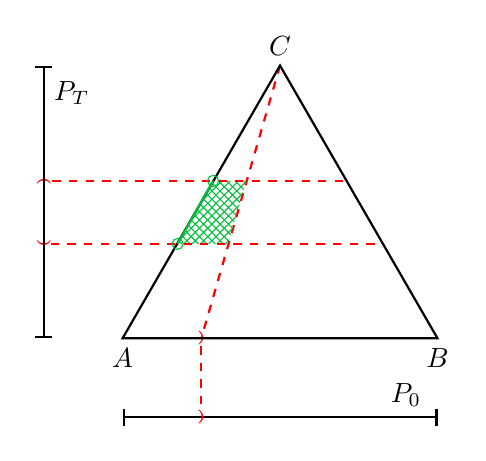
\begin{tikzpicture} %Triangle 2
\draw[thick, dashed,red] (0,{2*sqrt(3)})--(-1,0) node [font=\tiny\bf] {)};
\path[draw=none,pattern=crosshatch, pattern color=darkgreen] (-1.3,1.2)--(-0.66,1.2)--(-0.43,2)--(-0.86,2)--cycle;

\draw[thick] (-2,0)--(2,0)--(0,{2*sqrt(3)})--cycle;

\node (A) at (-2,0) [below] {\(A\)}; 
\node (B) at (2,0) [below] {\(B\)}; 
\node (C) at (0,{2*sqrt(3)}) [above] {\(C\)}; 

\draw[thick, dashed,red] (0.8,2)--(-3,2) node[font=\tiny\bf,rotate=90] {)};
\draw[thick, dashed,red] (1.2,1.2)--(-3,1.2) node[font=\tiny\bf,rotate=90] {(};

\draw[thick, dashed,red] (-1,-0.1)--(-1,-0.9);
\draw[thick, darkgreen] (-1.3,1.2)--(-0.85,2);

\draw[draw=darkgreen] (-1.3,1.2) circle (2pt);
\draw[draw=darkgreen] (-0.85,2) circle (2pt);

\draw[thick,|-|] (-3,0)--(-3,{2*sqrt(3)}) node[right,pos=0.9] {\(P_{T}\)};

\draw[thick,|-|] (-2,-1)--(2,-1) node[above,pos=0.9] {\(P_{0}\)} node[red,font=\tiny\bf] at (-1,-1) {)};
\end{tikzpicture}
}
\resizebox{0.3\textwidth}{!}{
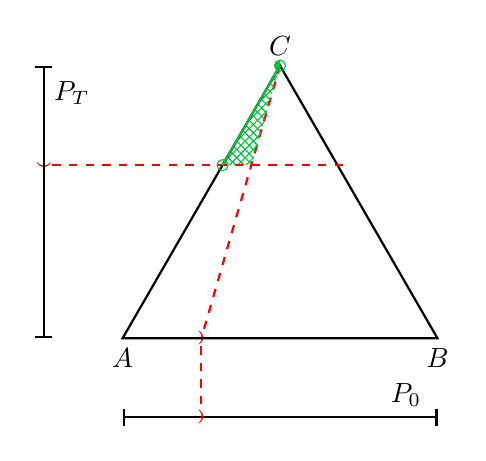
\begin{tikzpicture} %Triangle 1
\draw[thick, dashed,red] (0,{2*sqrt(3)})--(-1,0) node [font=\tiny\bf] {)};
\path[draw=none,pattern=crosshatch, pattern color=darkgreen] (-0.36,2.2)--(0,{2*sqrt(3)})--(-0.75,2.2)--cycle;

\draw[thick] (-2,0)--(2,0)--(0,{2*sqrt(3)})--cycle;

\node (A) at (-2,0) [below] {\(A\)}; 
\node (B) at (2,0) [below] {\(B\)}; 
\node (C) at (0,{2*sqrt(3)}) [above] {\(C\)}; 
\draw[thick, dashed,red] (0.8,2.2)--(-3,2.2) node[font=\tiny\bf,rotate=90] {(};
\draw[thick, dashed,red] (-1,-0.1)--(-1,-0.9);
\draw[thick, darkgreen] (-0.73,2.2)--(0,{2*sqrt(3)});

\draw[draw=darkgreen] (-0.73,2.2) circle (2pt);

\draw[draw=darkgreen] (0,{2*sqrt(3)}) circle (2pt);

\fill[darkgreen] (0,{2*sqrt(3)}) + (0, 2pt) arc (90:270:2pt);

\draw[thick,|-|] (-3,0)--(-3,{2*sqrt(3)}) node[right,pos=0.9] {\(P_{T}\)};

\draw[thick,|-|] (-2,-1)--(2,-1) node[above,pos=0.9] {\(P_{0}\)} node[red,font=\tiny\bf] at (-1,-1) {)};
\end{tikzpicture}
}
\resizebox{0.3\textwidth}{!}{
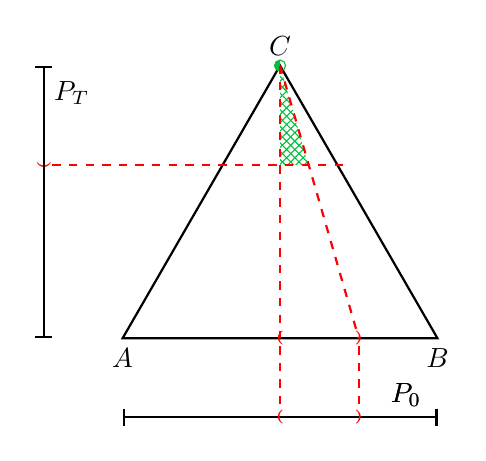
\begin{tikzpicture} %Triangle 1
\path[draw=none,pattern=crosshatch, pattern color=darkgreen] (0.36,2.2)--(0,{2*sqrt(3)})--(0,2.2)--cycle;

\draw[thick] (-2,0)--(2,0)--(0,{2*sqrt(3)})--cycle;

\node (A) at (-2,0) [below] {\(A\)}; 
\node (B) at (2,0) [below] {\(B\)}; 
\node (C) at (0,{2*sqrt(3)}) [above] {\(C\)}; 
\draw[thick, dashed,red] (0.8,2.2)--(-3,2.2) node[font=\tiny\bf,rotate=90] {(};

\draw[draw=darkgreen] (0,{2*sqrt(3)}) circle (2pt);

\fill[darkgreen] (0,{2*sqrt(3)}) + (0, 2pt) arc (90:270:2pt);

\draw[thick, dashed,red] (0,{2*sqrt(3)})--(1,0) node [font=\tiny\bf] {)};
\draw[thick, dashed,red] (0,{2*sqrt(3)})--(0,0) node [font=\tiny\bf] {(};

\draw[thick,|-|] (-3,0)--(-3,{2*sqrt(3)}) node[right,pos=0.9] {\(P_{T}\)};
\draw[thick,|-|] (-2,-1)--(2,-1) node[above,pos=0.9] {\(P_{0}\)};

\draw[thick, dashed,red] (1,-0.1)--(1,-0.9);
\draw[thick, dashed,red] (0,-0.1)--(0,-0.9);

\draw[thick,|-|] (-2,-1)--(2,-1) node[above,pos=0.9] {\(P_{0}\)}
node[red,font=\tiny\bf] at (1,-1) {)}
node[red,font=\tiny\bf] at (0,-1) {(};
\end{tikzpicture}
}
\caption{Exterior open patches. On the left is the facet patch, because it only touches a side (facet) of the simplex and not a corner. In the center is an exterior open patch where the facet component \(P_0\) is itself a facet patch (touching an edge and a corner), and on the right is an exterior open patch that touches a corner only because \(P_0\) is an interior open patch. Note that the point containing the corner at \(C\) in the middle and right diagram is only half filled because the patch contains some values where \(P(C) = 1\) and not others, depending on the relative probability between \(A\) and \(B\).}
\label{fig:exterior_open_patch}
\end{figure}

\begin{definition}
An \textit{open patch} is a subset of \(\text{RPF}(K)\) that is either an interior or exterior open patch.
\end{definition}

Now let the open patches be a basis for an open set thus defining a topology on \(\text{RPF}(K)\).

\begin{definition}
An \textit{open set} of \(\text{RPF}(K)\) is any (potentially infinite) union of open patches on \(\text{RPF}(K)\), or any finite intersection of open patches on \(\text{RPF}(K)\).
\end{definition}

\subsection{Compactness}

The following is sketch of the compactness proof for \(\text{RPF}(K)\) using open patches for illustrative purposes, as its compactness was already proven in \cite{paper}.

\begin{lemma}
\label{lem:withhold_possible_outcome}
Let \(h\) be an outcome, and let q be a number such that \(0 < q \leq 1\). The region of \(\text{RPF}(K)\) where the \(P(h) = q\) is isomorphic to \(\text{RPF}(K-1)\).
\end{lemma}

\begin{proof}
If \(P(h) > 0\) then it is in the anchored equivalence class of mutually possibility. If \(P(h) = 1\) then the outcome \(h\) can be appended above any function in \(\text{RPF}(K - 1)\), and if \(P(h) < 1\) then \(h\) can be appended into the anchored equivalence class of any function in \(\text{RPF}(K-1)\). In both cases, a separate \(h\) with a given absolute probability can be appended to anything in \(\text{RPF}(K-1)\) to produce an element of \(\text{RPF}(K)\), with all elements of \(\text{RPF}(K)\) accounted for.
\end{proof}

\begin{lemma}
\label{lem:change_one_anchor_outcome}
Let \(h\) be an outcome, and let \(P(h) > 0\). Given a number \(0 < q \leq 1\), there is a unique RPF \(P'\) which is equal to \(P\) when evaluated on outcomes \(\neq h\) and such that \(P'(h) = q\).
\end{lemma}

\begin{proof}
This will be a proof by construction. Let \(P'\) be the new distribution where \(h\) remains an anchor outcome, but its absolute probability has been changed to \(q\). For any anchor outcome \(a\), we set \(P'(a, h) = P(a, h) \cdot q \cdot P(a)^{-1} \)

For any non-anchor outcome \(b\), we note that \(P(b, h) = 0\) and therefore also \(P'(b, h) = 0\), otherwise \(b\) would now be possible relative to other anchors where it wasn't before.
\end{proof}

\begin{lemma}
\label{lem:open_anchor_outcome}
Let \(h\) be an outcome, and let \(P(h) > 0\). Any open patch of \(\text{RPF}(K)\) that contains \(P\), also contains, for some open interval on \(\mathbb{M}\) containing \(P(h)\), all the values \(P'\) constructed through lemma \ref{lem:change_one_anchor_outcome} by setting \(P'(h) = q\) for any \(q\) in that open interval.
\end{lemma}

This proof for \ref{lem:open_anchor_outcome} will be left open.

\begin{theorem}
\(\text{RPF}(K)\) is \textit{compact}, meaning that for every open cover of it, there is a finite subcover.
\end{theorem}

\begin{proof}
This is an inductive proof where we assume that the theorem is true for all \(k < K\) and then prove that it is true for \(K\).

If \(K \in {0, 1}\) then \(\text{RPF}(K)\) is finite and singular (either the empty RPF or unit RPF respectively). These are obviously compact. If \(K = 2\) then we have the topology of \(\mathbb{M}\) which is also compact (thanks to the \(\infty\) element).

Now we assume that \(K > 2\).

Consider the region of \(\text{RPF}(K)\) where a specific outcome is required to be the largest (or possibly ties for largest). In other words, for this special outcome \(h\), look at the region of \(\text{RPF}(K)\) where \(P(h', h) \leq  1\) for any other outcome \(h'\). There is one region for every outcome - \(K\)such regions overall - and collectively they cover \(\text{RPF}(K)\) but they are not disjoint. In fact, the uniform distribution belongs to all \(K\) regions!

If we can show that an open cover on \(\text{RPF}(K)\) has a finite subcover on a region, then it must have a finite subcover overall because there are a finite number of regions.

So consider one such region, and let \(h\) be the largest outcome from that region. \(h\) is an anchor element, which means that \(P(h, h') > 0\) for all \(h'\) when in fact it is \(\geq 1\). If \(P(h) = q\), then we know that \(\frac{1}{k} \leq q \leq 1\). By lemma \ref{lem:withhold_possible_outcome}, the rest of the distribution is isomorphic to \(\text{RPF}(K - 1)\) - and therefore compact by our inductive assumption. Therefore, there is a finite subcover covering all elements where \(P(h) = q\).

By lemma \ref{lem:open_anchor_outcome}, finite subcover will not just include cases where \(P(h) = q\), but will hold for some open interval around q as well.

So for each q where \(\frac{1}{K} \leq q \leq 1\), we have a finite subcover, with each subcover covering some open set around q. Because \([\frac{1}{K}, 1]\) is compact, all of these open sets around q have a finite subcover for the whole segment. This means that only finitely many of these q-based subcovers are required, and with each one being finite we have finitely many open sets for the entire region where \(h\) is the largest outcome.
\end{proof}

%\subsubsection*{References}
\begin{thebibliography}{20}

\bibitem{paper}Sklar, M. (2022) Relative Probability on Finite Sample Spaces

\end{thebibliography}

This document along with revisions is posted at github as https://github.com/maxsklar/relative-probability-finite-paper. See readme for contact information. Local Maximum Labs is an ongoing effort create an disseminate knowledge on intelligent computing.
\end{document}
